\documentclass[a4paper]{report}

% --- PACKAGES DE BASE ---
\usepackage[utf8]{inputenc}
\usepackage[T1]{fontenc}
\usepackage[french]{babel}
\usepackage[left=2.5cm, right=2.5cm, top=2.5cm, bottom=2.5cm]{geometry}

% --- GRAPHISMES ET MISE EN PAGE ---
\usepackage{graphicx}
\usepackage{float}
\usepackage{xcolor}
\usepackage{tikz}
\usepackage{background}
\usepackage{pdfpages}
\usepackage{wrapfig}
\usepackage{array}

% --- TITRES ET SOMMAIRE ---
\usepackage{titlesec}
\usepackage{tocloft}

% --- OUTILS SUPPLÉMENTAIRES ---
\usepackage{amsmath}
\usepackage{lipsum}
\usepackage{verbatim}
\usepackage[colorlinks=true, linkcolor=blue, citecolor=green]{hyperref}

% --- CONFIGURATION LISTINGS (CODE) ---
\usepackage{listings}
\definecolor{codegreen}{rgb}{0,0.6,0}
\definecolor{codegray}{rgb}{0.5,0.5,0.5}
\definecolor{codepurple}{rgb}{0.58,0,0.82}
\definecolor{backcolour}{rgb}{0.95,0.95,0.92}

\lstdefinestyle{pythonstyle}{
    backgroundcolor=\color{backcolour},
    commentstyle=\color{codegreen},
    keywordstyle=\color{blue},
    numberstyle=\tiny\color{codegray},
    stringstyle=\color{codepurple},
    basicstyle=\ttfamily\footnotesize,
    breaklines=true,
    captionpos=b,
    keepspaces=true,
    numbers=left,
    numbersep=5pt,
    showspaces=false,
    showstringspaces=false,
    showtabs=false,
    tabsize=2,
    language=Python,
    literate={é}{{\'e}}1 {è}{{\`e}}1 {à}{{\`a}}1 {ç}{{\c{c}}}1 {œ}{{\oe}}1 {ù}{{\`u}}1 {É}{{\'E}}1 {È}{{\`E}}1 {À}{{\`A}}1 {°}{{$^\circ$}}1
}
\lstset{style=pythonstyle}

% --- CONFIGURATION DES TITRES ---
\titlespacing*{\chapter}{0pt}{-20pt}{30pt}
\titleformat{\chapter}[display]
  {\normalfont\Huge\bfseries} % Taille pour "Chapitre X"
  {\chaptertitlename\ \thechapter}
  {10pt}                      % Espace entre le numéro et le titre (réduit ici)
  {\huge}                     % Taille pour le nom du titre (modifié de \Huge à \huge)

\renewcommand{\contentsname}{Table des matières}

% --- DÉBUT DU DOCUMENT ---
\begin{document}

% 1. Page de garde (via PDF externe)
\backgroundsetup{contents={}}

\includepdf[pages=-, fitpaper=true]{Template.pdf}

% 2. Configuration du fond pour le reste du document
\backgroundsetup{
    scale=1,
    angle=0,
    opacity=1,
    color=black,
    contents={
        \begin{tikzpicture}[remember picture,overlay]
        \node at ([xshift=-0.8in,yshift=0.8in] current page.south east) {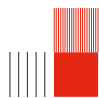
\includegraphics[scale=0.8]{images/pattern.png}};
        \end{tikzpicture}
    }
}

% 3. Remerciements
\clearpage
\thispagestyle{empty}
\vspace*{\fill}
\section*{Remerciements}
\addcontentsline{toc}{chapter}{Remerciements}
Ce projet multidisciplinaire n'aurait pu voir le jour sans l'aide de...
\vspace*{\fill}

% 4. Abstract
\clearpage
\thispagestyle{empty}
\vspace*{\fill}
\section*{Abstract}
\addcontentsline{toc}{chapter}{Abstract} % Corrigé ici
Ce document est le rapport final du projet... 
\vspace*{\fill}

% 5. Sommaire et Contenu
\clearpage
\tableofcontents

\chapter{Introduction}

\section{Contexte}
Dans le cadre du projet multidisciplinaire de 4ème du Génie physique de l'INSA Toulouse, nous devons modéliser les lentilles électrostatiques quadrupolaires 
d'un FIB (Focused Ion Beam) en utilisant une méthode mathématique appelée la méthode des éléments de frontière. Pour ce faire, nous devons écrire un code Python 
en utilisant notamment la bibliothèque BEMPP. Afin de pouvoir réaliser cette entreprise, il est nécessaire de comprendre l'optique des particules chargées dans le contexte
de lentilles quadrupolaires. 

\section{Fondemement théorique}

\subsection{L'optique des particules chargés}

L'optique est une science divisée en deux domaines majeurs. L'optique photonique étudie le comportement de la lumière
 à travers des lentilles ou des miroirs. Cette technologie est ulisé dans les microscopes classiques, les télescopes
 ou les apareils photos.
Cependant, la résolution de ces systèmes rencontre une limite physique : la diffraction.

En effet la résolution d'un systeme optique définit la capacité à distinguer deux points à distance proche.La résolution
peut s'exprmier avec le critère dritère de Rayleigh
\[
d = \frac{1.22 \times \Lambda}{n\sin(\alpha)}
\]

avec :

\begin{itemize}
    \item $\lambda$ est la longueur d'onde de la particule.
    \item $n$ est l'indice de réfraction du milieu.
    \item $\alpha$ est l'angle de demi-ouverture du faisceau.
\end{itemize} 

 Or la lumière possède une longueur d'onde entre 400 et 800 nm,
paramètre limitant la résolution des systèmes optiques. 

L'optique des particules chargé permet de s'affranchir de cette limite. Selon de Broglie, la longueur d'onde d'une
particule chargé depend de sa quantité de mouvement :

\[
\lambda = \frac{h}{mv}
\]

Pour des particules accélérées, la longueur d'onde devient extrêmement petite. 
Cette propriété permet de réduire  les effets de la diffraction.

Applications et instrumentation

LL'optique des particules chargées permet de maîtriser la trajectoire de faisceaux d'électrons ou d'ions. 
Des champs électrostatiques ou magnétiques agissent comme des lentilles. 
Cette discipline a permis de créer de 
nombreux instruments comme  les SEM (Scanning electron microscop = 
microscope électronique à balayage) et les FIB (focused ion beam = faisceau d’ions focalisé).
Ces outils sont 
utilisés dans de nombreuses disciplines comme la médecine ou la microélectronique.  
Plus spécifiquement, un FIB est composé de plusieurs étages dont notamment des 
lentilles. En effet, celles-ci permettent de guider la trajectoire du faisceau ionique au sein de 
l’instrument et de corriger les différentes aberrations de celui-ci. Il est donc primordial de 
comprendre et maîtriser ces objets afin de rendre le FIB le plus performant possible.  

\begin{figure}[H]
\centering
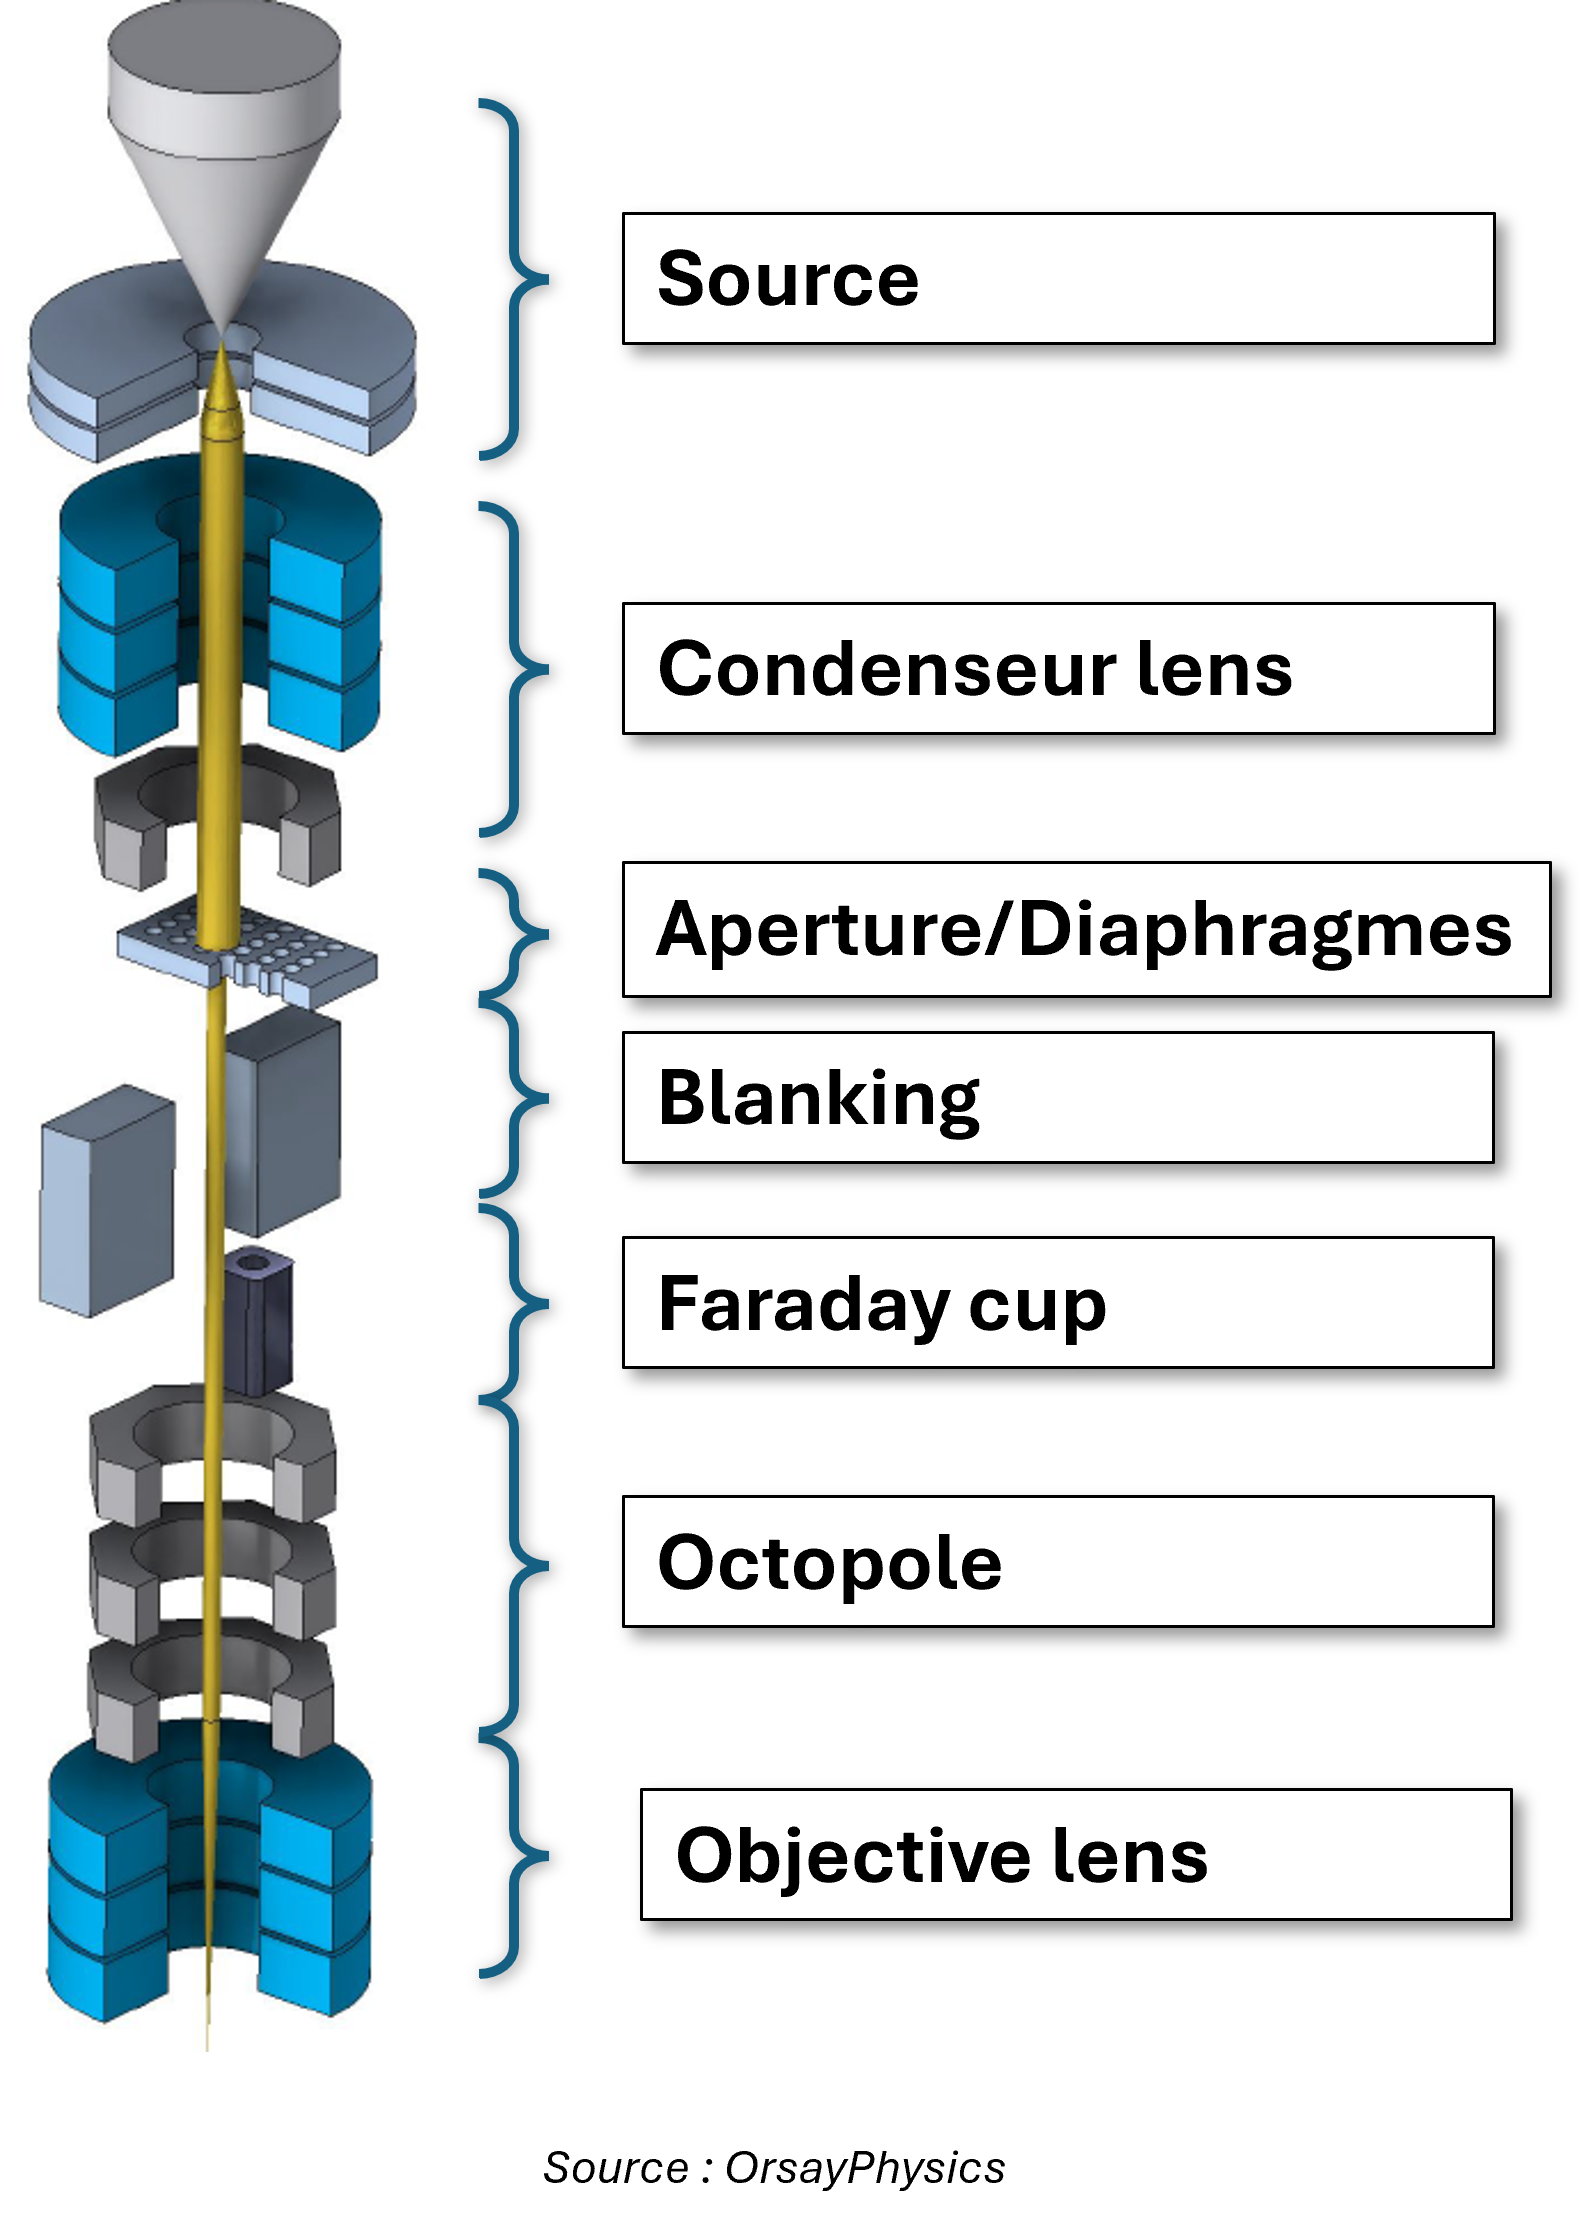
\includegraphics[width=0.3\linewidth]{images/Schema_Colonne_FIB_OP.png} 
\caption{Schéma d’un FIB}
\label{fig:fib}
\end{figure}


Comme évoqué précédemment, les lentilles permettent de guider la trajectoire du faisceau 
ionique. Il existe plusieurs types de lentilles: les lentilles électrostatiques et les lentilles 
magnétiques. Dans le cas que nous étudions, le FIB est composé de lentilles 
électrostatiques.  
Ces lentilles électrostatiques peuvent présenter différentes configurations. On parle en effet 
de lentilles rondes/monopolaires (un seul potentiel), de lentilles dipolaires (deux potentiels), 
de lentilles quadrupolaires (quatres potentiels), etc. 

\subsection{Principe de correction d'aberration}
L'usage de particules chargées réduit l'impact de la diffraction.
 Cependant, la résolution reste limitée par des aberrations liées aux imperfections des champs. 
 On distingue deux types principaux d'aberrations : les aberrations chromatiques, liées à la dispersion en énergie des particules, 
 et les aberrations géométriques.

Parmi les aberrations géométriques, on trouve notamment l'aberration sphérique, 
le coma, l'astigmatisme ou la distorsion. Ce rapport se concentre sur l'aberration sphérique.
 Ce défaut traduit le fait que les particules s'éloignant de l'axe optique sont focalisées plus fortement que les particules centrales.
  Il en résulte un élargissement du point focal dans le plan image,



\begin{figure}[H]
\centering
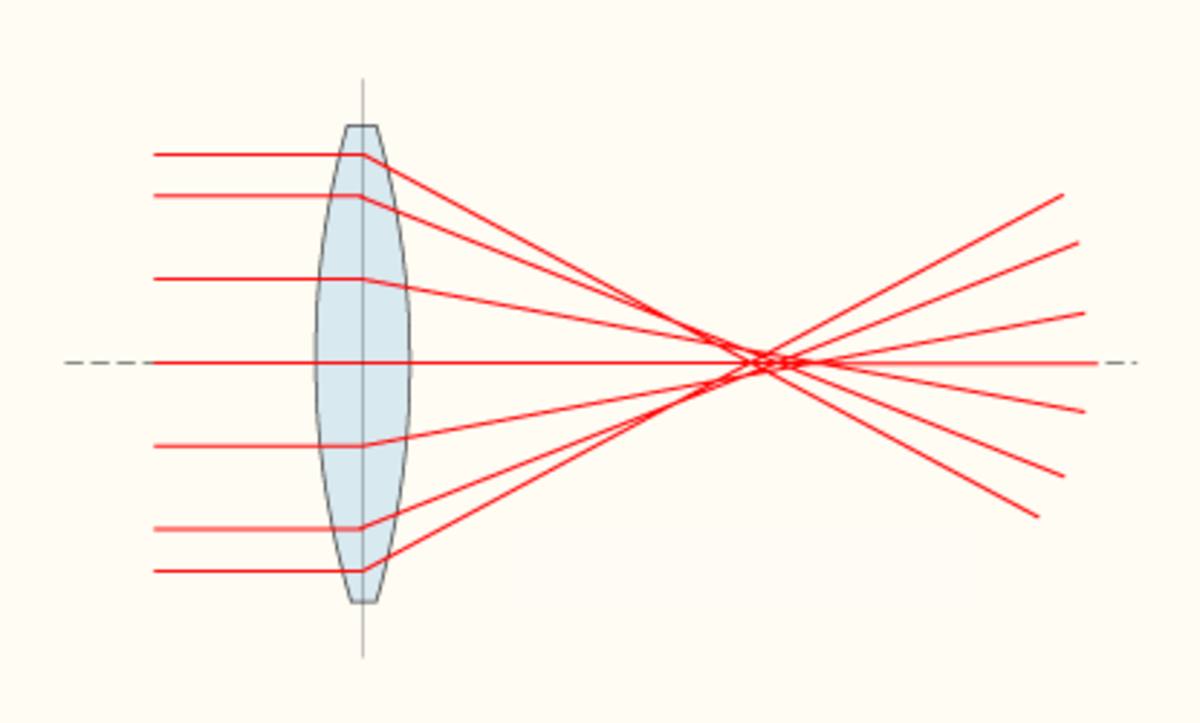
\includegraphics[width=0.3\linewidth]{images/aberation_spherique.png}
\caption{abérration sphérique }
\label{fig:abberation}
\end{figure}

La méthode classique pour corriger l'aberration sphérique utilise des correcteurs multipolaires.
 La superposition de champs quadrupolaires et octopolaires permet de compenser ce défaut.(mettre pourquoi)
 Cependant, l'alignement de ces nombreux étages représente un défi technique majeur.

\subsection{Le quadrupole d'okayama}

L'équipe de S. Okayama a travailler sur nouveau moyen de correction. Ce système évite l'utilisation d'électrodes octopolaires dédiées. 
En combinant un champ rond créer par une aperture et un champ quadrupolaire, un champ octopolaire apparaît naturellement. 
Ce champ est dit « auto-aligné », ce qui simplifie grandement la conception et le réglage du correcteur.


\chapter{Théorie physique}
\section{Principe de moindre action}
En optique des particules chargées, l'équivalent du principe de Fermat est le principe de moindre action.
Celui-ci s'exprime comme 
\[
\delta S = \int_{S0}^{S1} \vec{p}\,\frac{\vec{r}}{dS} \, \mathrm{d}s = 0
\]
\\
Ce principe peut être réecrit en utilisant l'indice optique. On a alors 
\[
\delta S = \int_{S0}^{S1} \mu\,\mathrm{d}z = 0
\]
\\
Comme le quadrupole que nous utilisons est composé UNIQUEMENT de lentilles électrostatiques, on peut écrire
\[
\mu = \sqrt{\phi(1+(x')^2 + (y')^2)}
\]
avec $\mu$ l'indice optique, $\phi$ le potentiel électrostatique et x' et y' les dérivées de x et y par
rapport à z.
\\
\\
Afin de pouvoir retrouver la trajectoire des particules chargées qui passent à travers le système, il faut 
retrouver l'indice optique du système. Cela est faisable en retrouvant le potentiel électrostatique dans tout le volume du
système et la vitesse des particules dans les directions x et y. 

\section{Equations d'Euler-Lagrange}
Les équations d'Euler-Lagrange sont des équations équivalentes au principe de moindre action, sous forme 
différentielle. On peut ainsi noter 
\[
\frac{\partial \mu }{\partial x}-\frac{d}{dz}\left(\frac{\partial \mu }{\partial x'}\right)=0
\]
\[
\frac{\partial \mu }{\partial y}-\frac{d}{dz}\left(\frac{\partial \mu }{\partial y'}\right)=0
\]

\section{Extraction du potentiel}
Afin de pouvoir retrouver le potentiel électrostatique en tout point du volume du système, on utilise une 
méthode mathématique: la méthode des éléments de frontières. En anglais, cette méthode se nomme Boundary 
Element Method (BEM). 
\\
\\
{\color{red}
--> Il faut détailler mais je sais pas quoi dire }
\\
\\
Une fois le potentiel extrait en tout point de l'espace, il est utile de décomposer celui-ci afin de pouvoir séparer les 
différentes composantes en fonction de leur dépendance aux différents ordres de x et y. On peut montrer que le potentiel s'exprime 
alors comme 

\[
\boxed{
\phi ({\color{red}r},{\color{blue}\theta},{\color{green}z})= \sum\limits_{\nu =0}^{\infty}
\sum\limits_{\lambda=0}^{\infty} \frac{(-1)^{\lambda}\times (\nu !)}{4^{\lambda}\times \lambda !\times (\lambda +\nu)!}
\times {\color{red}r}^{\nu +2\lambda} \times \left(\Phi_{\nu {r}}^{[2\lambda]}({\color{green}z})\times cos(\nu{\color{blue}\theta}) \right)
}
\]
\\
En injectant l'expression précédente dans les équations d'Euler-Lagrange, on obtient les équations différentielles suivantes, appelées équations de la trajectoire
\[
x''(z) + \frac{\phi'_0(z)}{2\phi_0}x'(z) + \left( \frac{\phi_0''(z)}{4\phi_0(z)} -
\frac{\phi_2(z)}{\phi_0(z)}\right) x(z) = 0
\]

\[
y''(z) + \frac{\phi'_0(z)}{2\phi_0}y'(z) + \left(\frac{\phi_0''(z)}{4\phi_0(z)} +
\frac{\phi_2(z)}{\phi_0(z)}\right) y(z) = 0
\]
\\
\\
Comme leur nom l'indique, la  résolution des équations suivantes à l'aide de la méthode mathématique Runge-Kutta 4, on retrouve la trajectoire des 
particules chargées à travers le système. 

\chapter{Application}
Le but de ce projet multidisciplinaire est de modéliser un quadrupole électrostatique. Pour cela, plusieurs étapes clés sont nécessaires: modélisation de la géométrie, extraction du 
potentiel électrostatique, décomposition du potentiel et résolution des équations de la trajectoire. 
\begin{figure}[H]
\centering
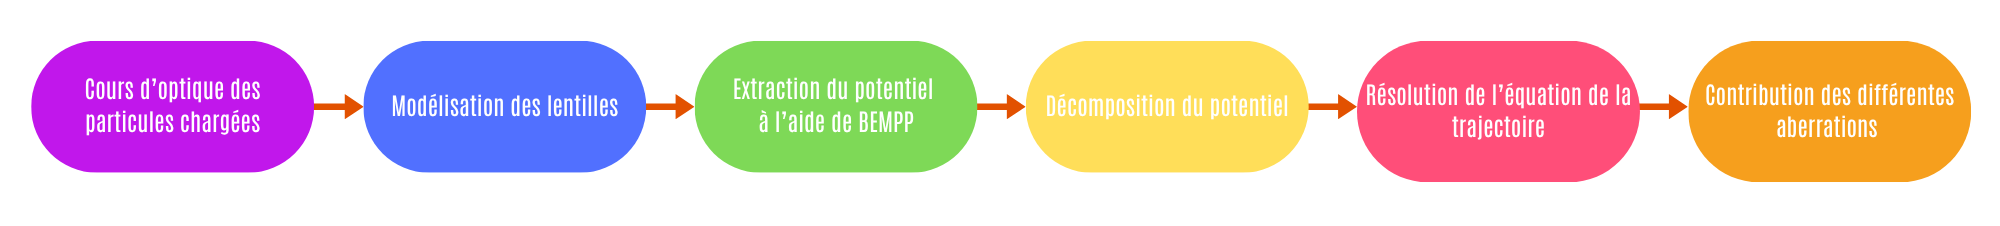
\includegraphics[width=1\linewidth]{images/Logigramme.png} 
\caption{Logigramme présentant les différentes étapes du projet}
\label{fig:Logigramme}
\end{figure}
\section{Modélisation du quadrupole d'Okayama}
Afin de pouvoir utiliser la méthode des éléments de frontière, il faut mailler la géométrie du quadrupole que nous souhaitons modéliser. Ce maillage est fait en utilisant une
extension en bibliothèque Python du générateur de maillage open-source Gmsh.
\\
\\
{\color{red}
--> Penser à créditer}
\\
\\
Au début du projet, nous nous sommes appuyées sur le projet multidisciplinaire de Niels BRUN et Paul BESNARD. Le but de ce projet était de modéliser 
des lentilles de Einzel. Ces lentilles sont trois électrodes circulaires trouées au centre. Les électrodes extérieures sont à la masse tandis que 
l'électrode du centre est polarisée. Ces lentilles servent dans le système de lentilles condenseurs. 
Afin de prendre en main la bibliothèque Gmsh, nous avons modélisé des lentilles de Einzel.

\begin{figure}[H]
\centering
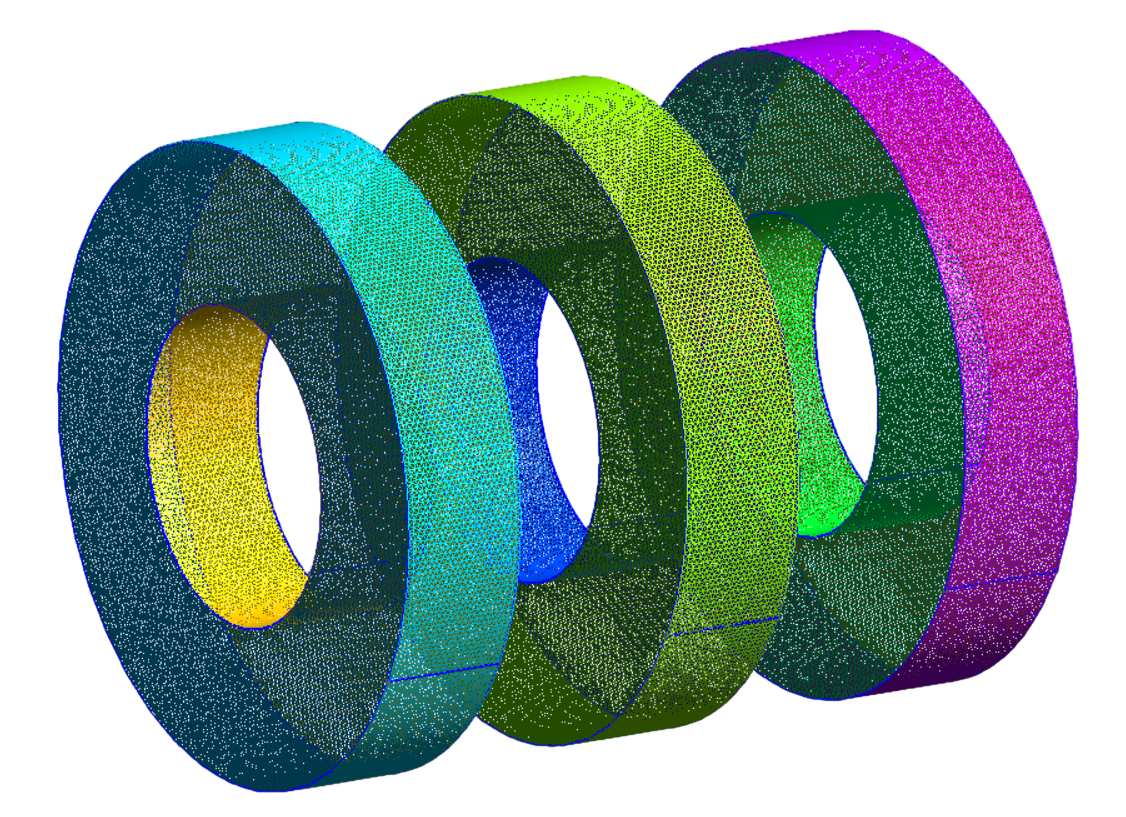
\includegraphics[width=0.4\linewidth]{images/Maillage Einzel.png} 
\caption{Maillage de lentille de Einzel avec Gmsh}
\label{fig:maillage_einzel}
\end{figure}

Une fois cette bibliothèque Pyhton maitrisée, nous avons pu passer à la modélisation et au maillage du quadrupole d'Okayama. Celui-ci est composé
de trois parties différentes: les électrodes cylindriques, les apertures circulaires et le shield. {(\color{red} doit on mettre ces mots en français?)}
Au centre du quadrupole se situent les quatres électrodes cylindriques. Celle-ci sont polarisées inversement polarisée par paires: toutes les électrodes
ont le même potentiel à un signe près. Ces électrodes permettent de focaliser le rayon selon une direction et le défocaliser selon une autre.
Les apertures servent à {(\color{red} je sais pas quoi dire ici)}
Le shield quand à lui sert à isoler le quadrupole afin de représenter un système réaliste car le quadrupole est toujours enfermé dans la colonne de 
l'intrument sur lequel il est installé. 

\begin{figure}[H]
\centering
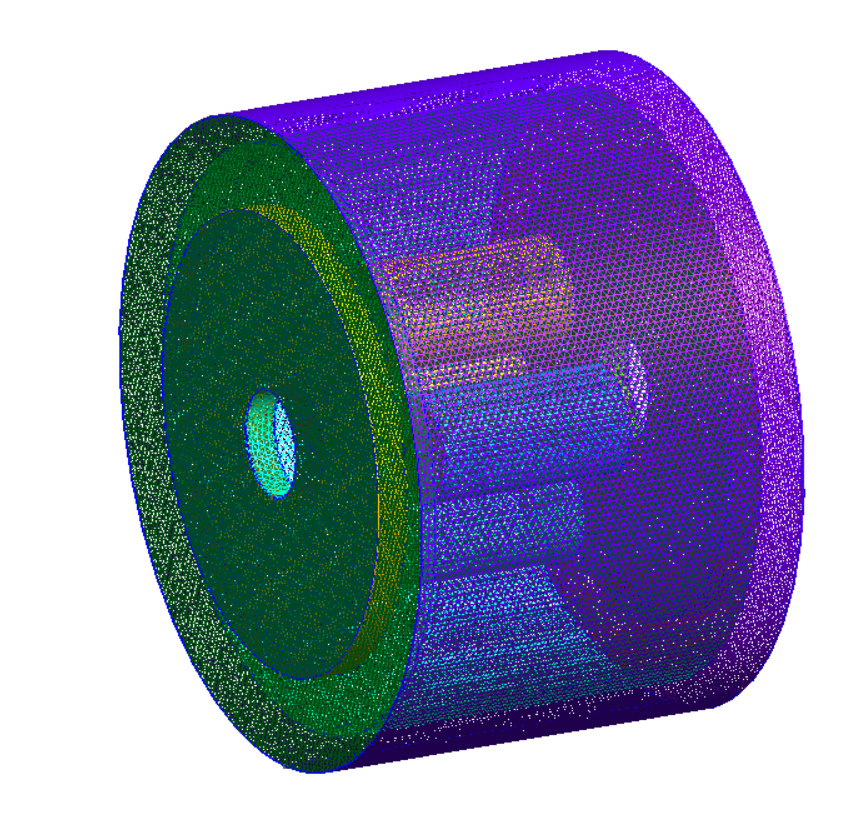
\includegraphics[width=0.3\linewidth]{images/Maillage de biais incliné.png} 
\caption{Maillage du quadrupole (vue complète)}
\label{fig:maillage_quad_complet}
\end{figure}

\begin{figure}[H]
\centering

\begin{minipage}{0.4\textwidth}
    \centering
    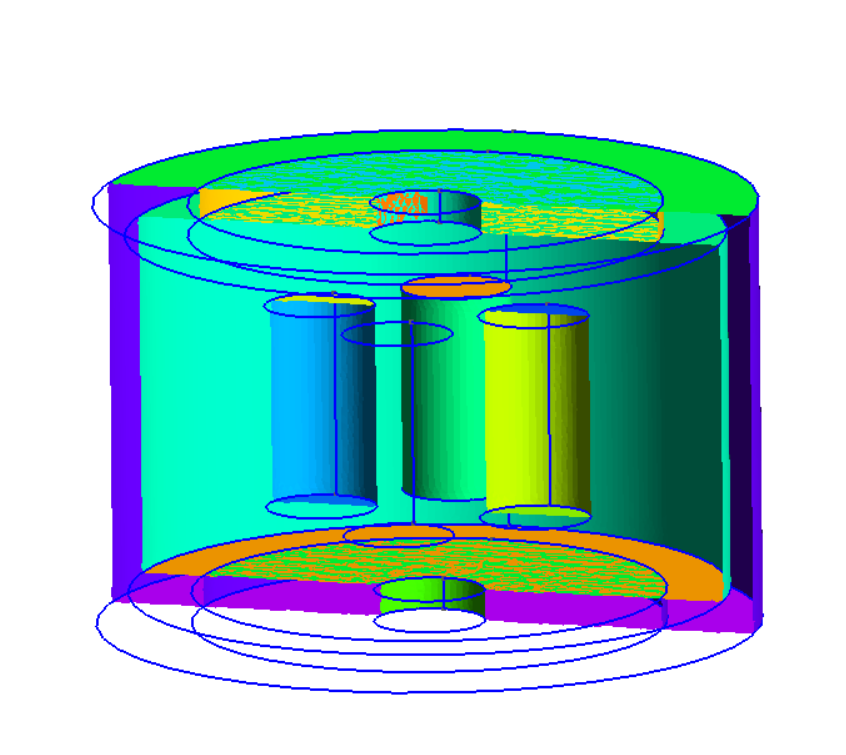
\includegraphics[width=\linewidth]{images/Coupe en longueur.png}
    \caption{Vue en coupe dans la longueur du quadrupole}
    \label{fig:coupe_quad}
\end{minipage}
\hspace{2cm}
\begin{minipage}{0.4\textwidth}
    \centering
    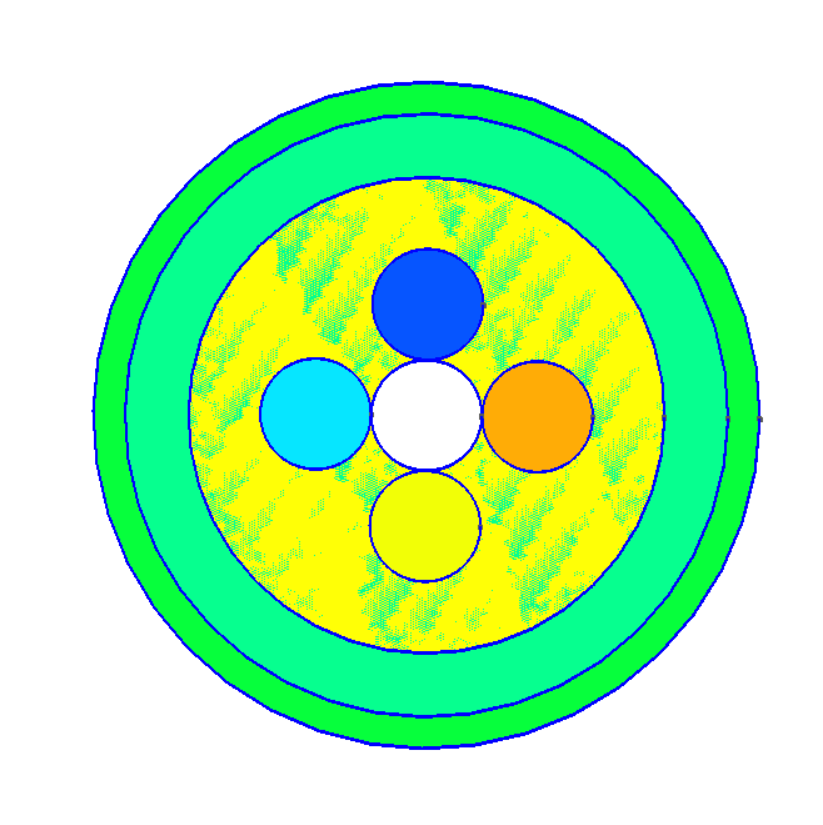
\includegraphics[width=\linewidth]{images/Coupe de face.png}
    \caption{Vue en coupe de face du quadrupole}
    \label{fig:shield_quad}
\end{minipage}

\end{figure}

\end{document}